\section{Appendix: Misrepresentation of Cluster Salience}\label{sec:appendix_false_pos}

\subsection{Effects of PCA Pre-processing}
It is common practice to pre-process a t-SNE input by reducing the dimension with PCA \citep{kobak2019art}. In light of the results of Section \ref{sec:mis_clusters}, it is natural to ask how this PCA pre-processing step plays with t-SNE's additive invariance. Figures \ref{fig:PCA_preprocessing} and \ref{fig:PCA_preprocessing_example} provide evidence that, even if the input is pre-processed with PCA, there exist a sequence of datasets with similar visualizations but vastly different input cluster strengths as measured via silhouette score and aspect ratio. %Thus, short of the most extreme cases where PCA helps, the output may still be untrustworthy even when using PCA pre-processing.


%The goal of this technique is to merge PCA's ability to recover global structure with t-SNE's focus on local structure. One may hope that this improved global structure preservation may help detect exaggerated clusters; however, we demonstrate that this method is insufficient. 


In both figures, the dataset at hand is $1000$ points sampled from a mixture of two Gaussians in $100$ dimensions. Algorithm \ref{alg:impostor} is applied at various strengths to vary the silhouette score and aspect ratio.


\begin{figure}[h!]
    \centering
    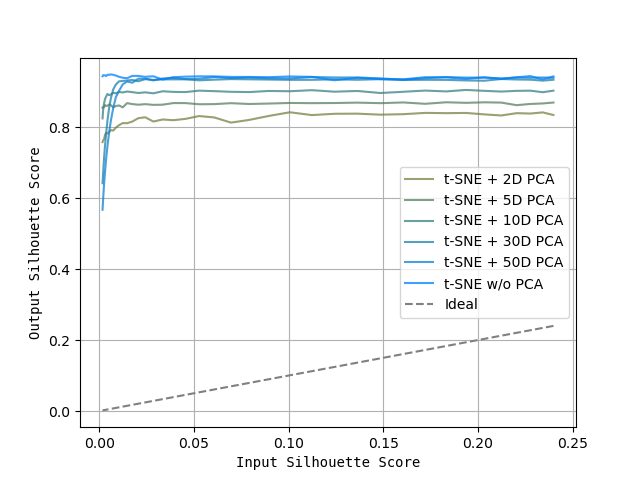
\includegraphics[width=0.6\linewidth]{images/appendix_figs/PCA_Preprocessing.png}
    \caption{\small Effect of PCA Pre-processing on Silhouette Score: input versus t-SNE output silhouette score using various levels of PCA pre-processing. 
}
    \label{fig:PCA_preprocessing}
\end{figure}

%Example outputs of t-SNE with PCA pre-processing on a mixture of two Gaussians.
\begin{figure}[h!]
    \centering
    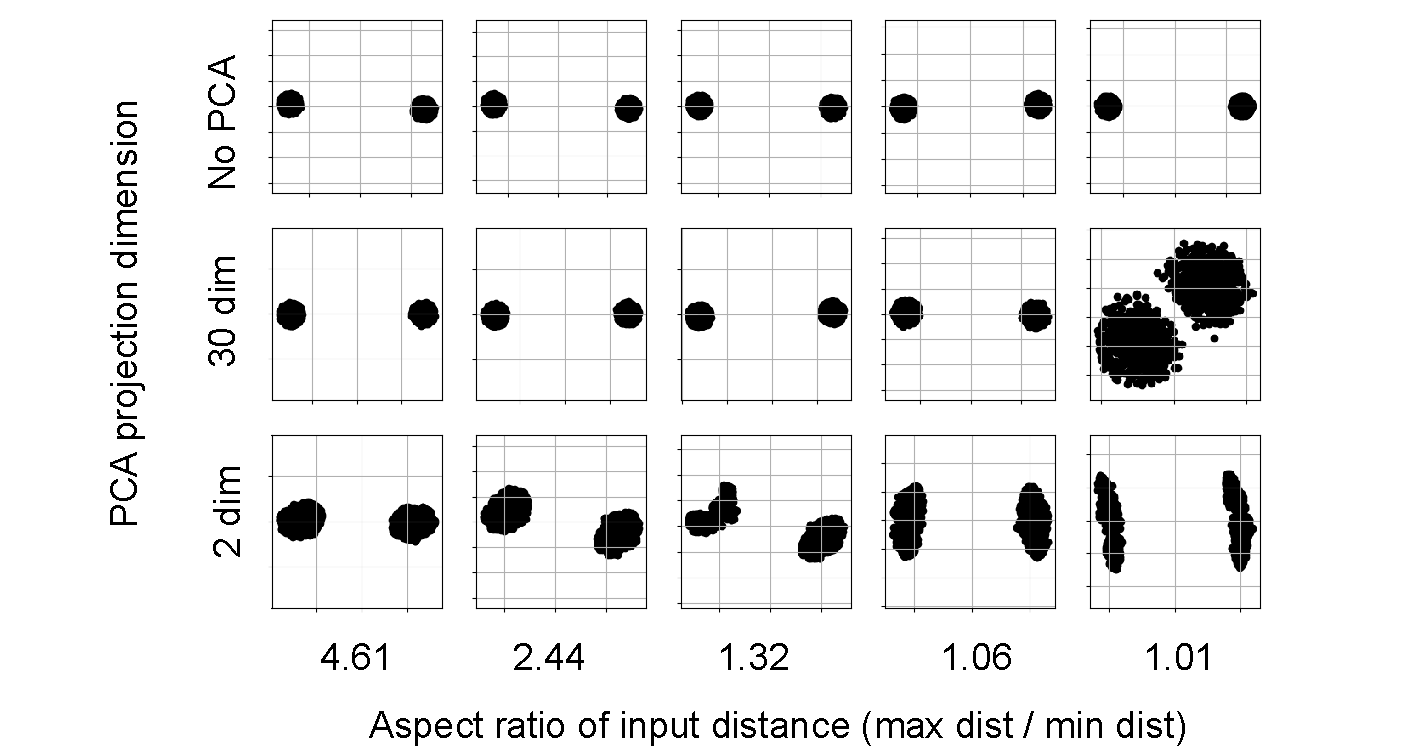
\includegraphics[width=0.95\linewidth]{images/appendix_figs/PCA_Preprocessing_example.pdf}
    \caption{\small Effect of PCA pre-processing on visualization. Note that without PCA, t-SNE is perfectly additively invariant, whereas this is not the case with PCA pre-processing.} \label{fig:PCA_preprocessing_example}
    
\end{figure}


\subsection{Additional Experiments}
%\todo[inline]{Make Figure 6 appear here.}
\iffalse
\begin{figure}
    \centering
    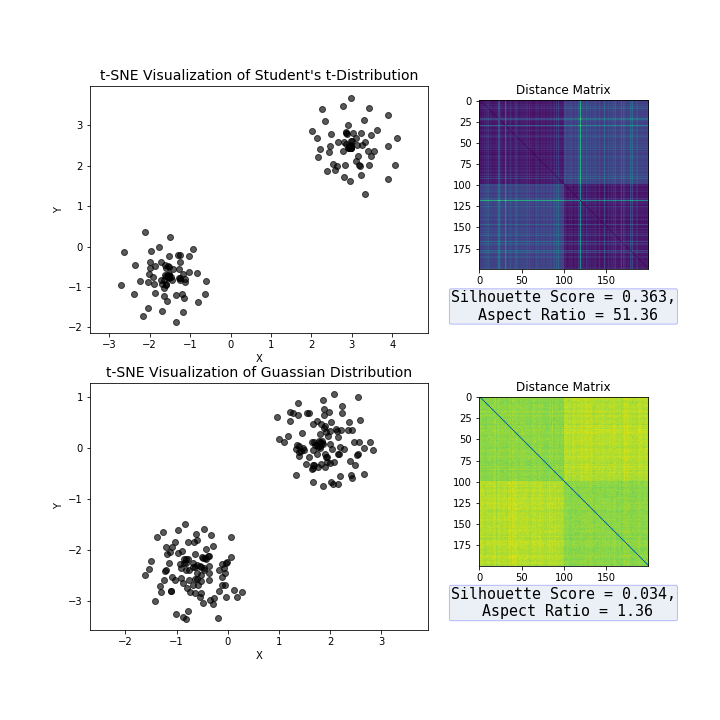
\includegraphics[width=0.49\linewidth]{images/Same_Output_Diff_Input_in_same_dim_9_19_25.png}
    \caption{Mixture of Gaussians of Increasing Dimension.} \label{fig:DiffIn_SameOut}
    \todo[inline]{Update caption.}
    The t-SNE visualization and interpoint distance matrix of 50 points sampled from $N\left(\vec{0}, \frac{1}{d^{3/4}}I_d\right)$ and 50 points sampled from $N\left(\vec{e}_1,  \frac{1}{d^{3/4}}I_d\right)$ for $d \in [100, 1000, 10000].$ Notice that as the dimension increases, the interpoint distance matrix of the input approaches a simplex but the t-SNE visualization becomes more clustered.
\end{figure}
\fi

In Figure \ref{fig:higher_dim_tighter_clusters}, we plot a sample from a mixture of two Gaussians in 250, 500, 1000, 2000, and 4000 dimensions. Notice that as the dimension of the Gaussian increases, the interpoint distance matrix of the input points (bottom) approaches a simplex but the t-SNE corresponding visualization (top) remains qualitatively unchanged. 

\begin{figure}[h!]
    \centering
    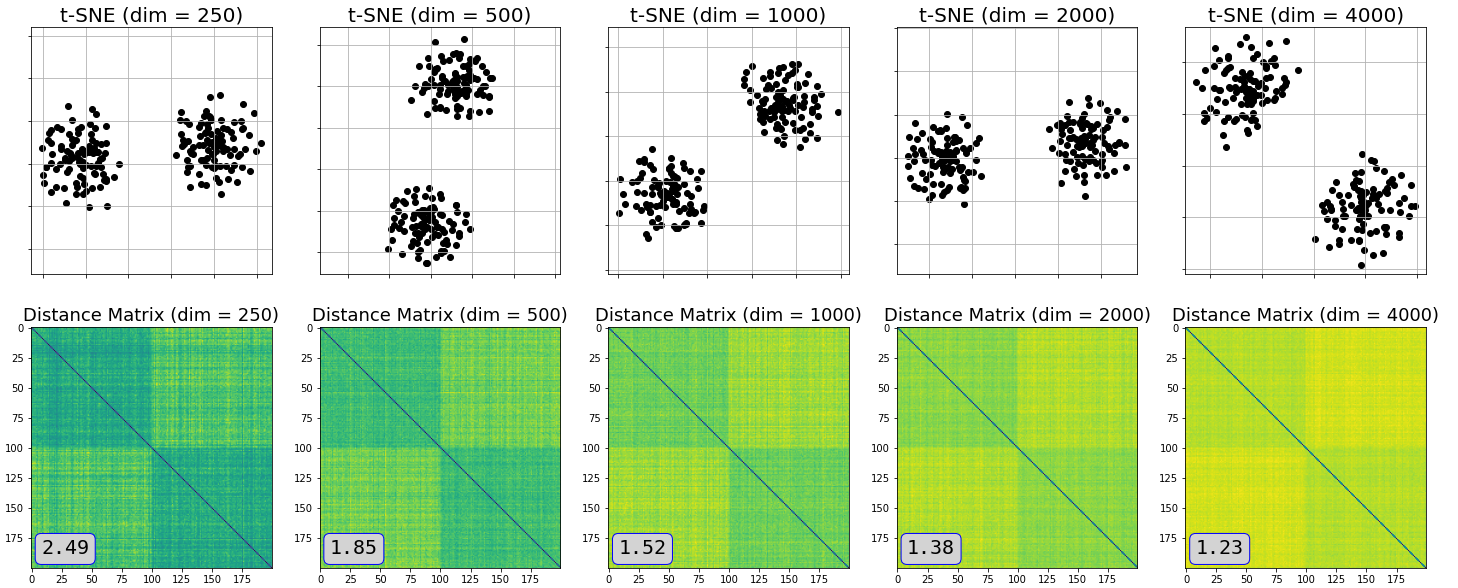
\includegraphics[width=\linewidth]{images/appendix_figs/Same_Output_Diff_Input_9_22_25.png}
    \caption{\small t-SNE's interplay with the concentration of measure phenomenon. The bottom left number in the plots show the aspect ratio (i.e.\ largest interpoint distance to the smallest interpoint distance).
 %   \todo[inline]{Decide whether to keep or remove this figure.}]
}\label{fig:higher_dim_tighter_clusters}
\end{figure}


Figure \ref{fig:poison_point_scaling} below shows that the effects of adding a poison point persists even with larger Gaussian clustered datasets. 

\begin{figure}[h!]
    \centering
    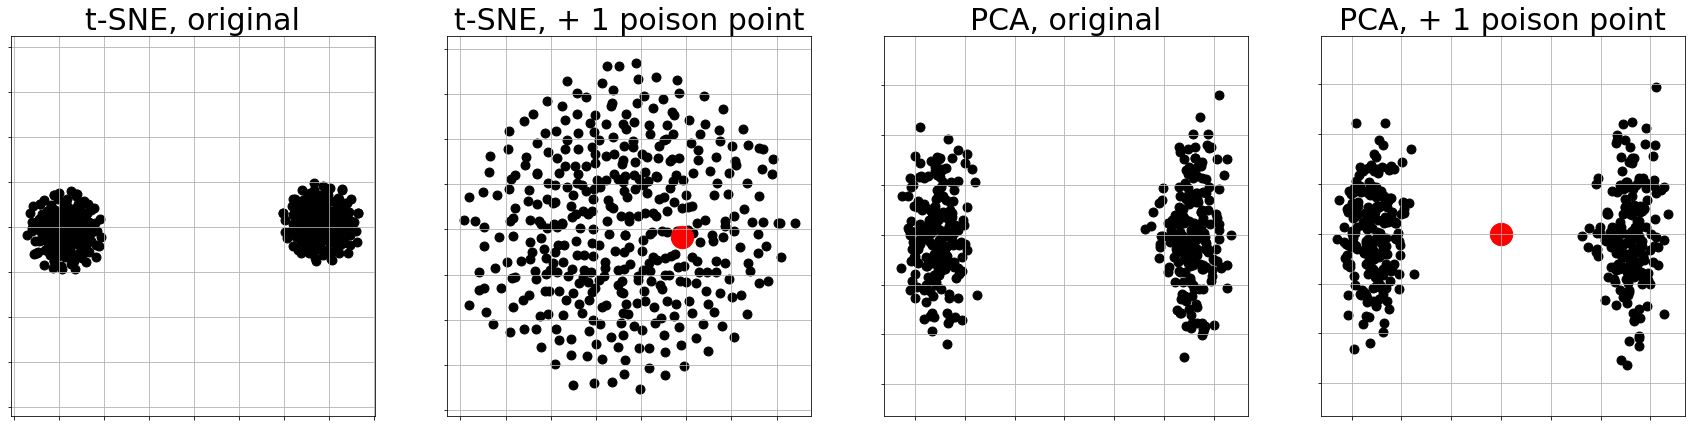
\includegraphics[width=0.9\linewidth]{images/outlier_figs/one_pt_perturb.png}
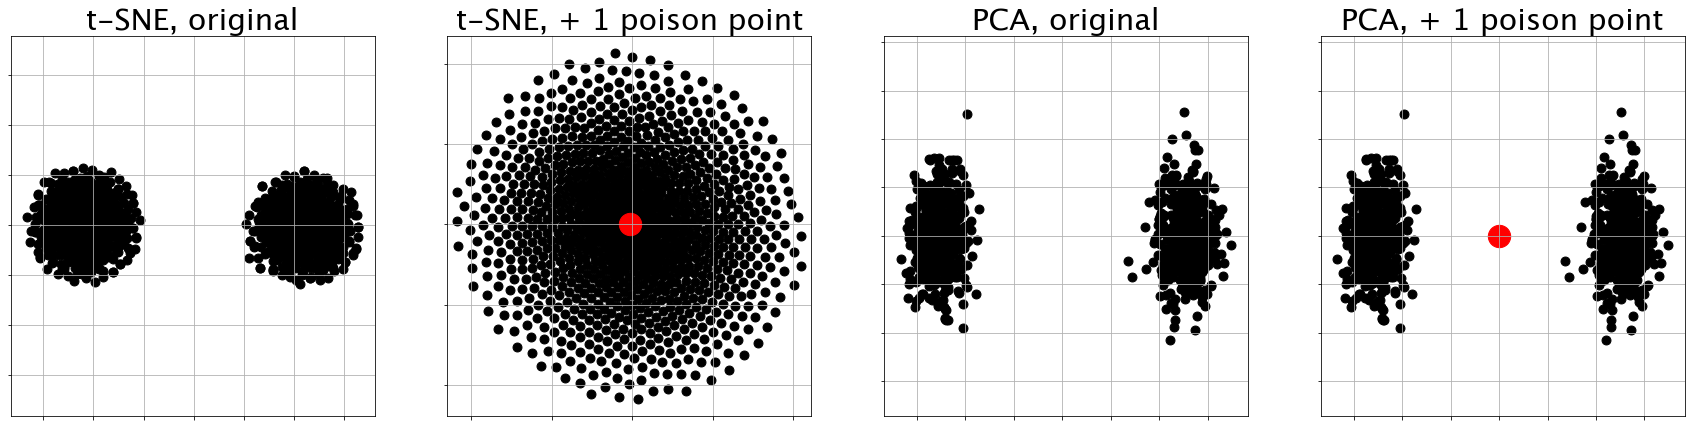
\includegraphics[width=0.9\linewidth]{images/poison_point/one_pt_perturb_1000.png}
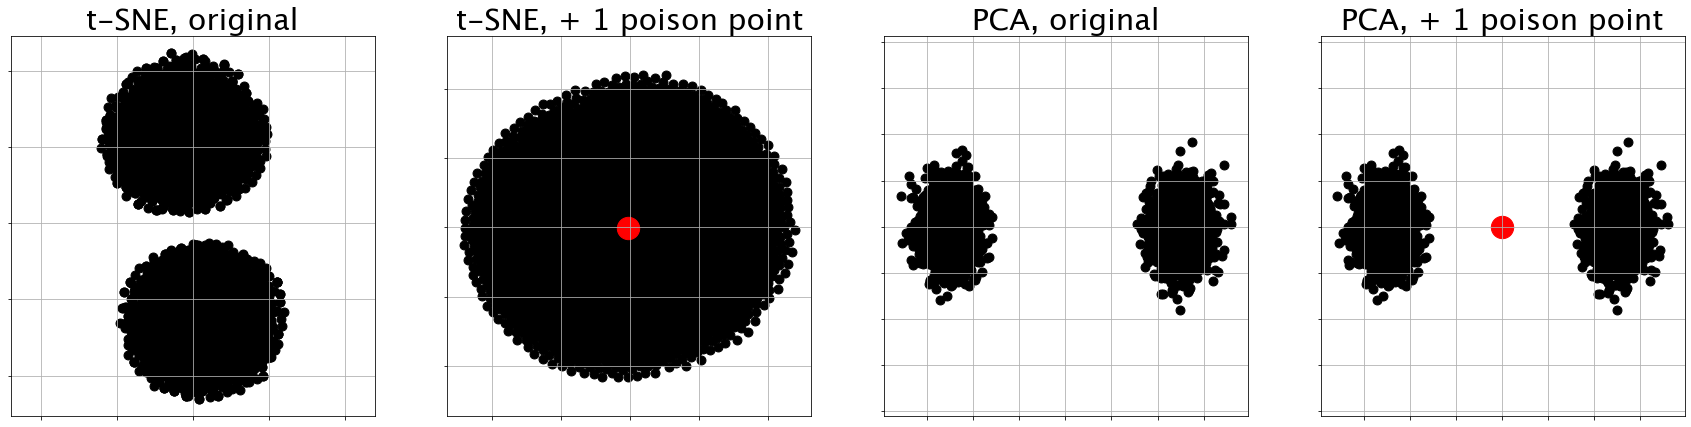
\includegraphics[width=0.9\linewidth]{images/poison_point/one_pt_perturb_5000.png}

    
    \caption{\small Top row: 400 total points, Middle row: 1000 total points, Bottom Row: 5000 total points}
    \label{fig:poison_point_scaling}
\end{figure}

\newpage 

Figure \ref{fig:poison_point_thm} provides an experimental demonstration of Theorem \ref{thm:poison_point}. 

\begin{figure}[h!]
    \centering

\includegraphics[width=0.97\linewidth]{images/poison_point/thm7.png}
    \caption{{\small An experimental demonstration of Theorem \ref{thm:poison_point}. This shows that \(X_0\), the un-clustered input (with silhouette score of \(0\)), has an un-clustered t-SNE output (first panel), while \(X_1\), the clustered input (with silhouette score around \(0.422\)), has a very clustered t-SNE output (third panel). However, with the insertion of the poison point, the t-SNE outputs are similarly un-clustered (second and fourth panels).}}
    \label{fig:poison_point_thm}
\end{figure}


%\begin{figure}[h!]
%    \centering
%    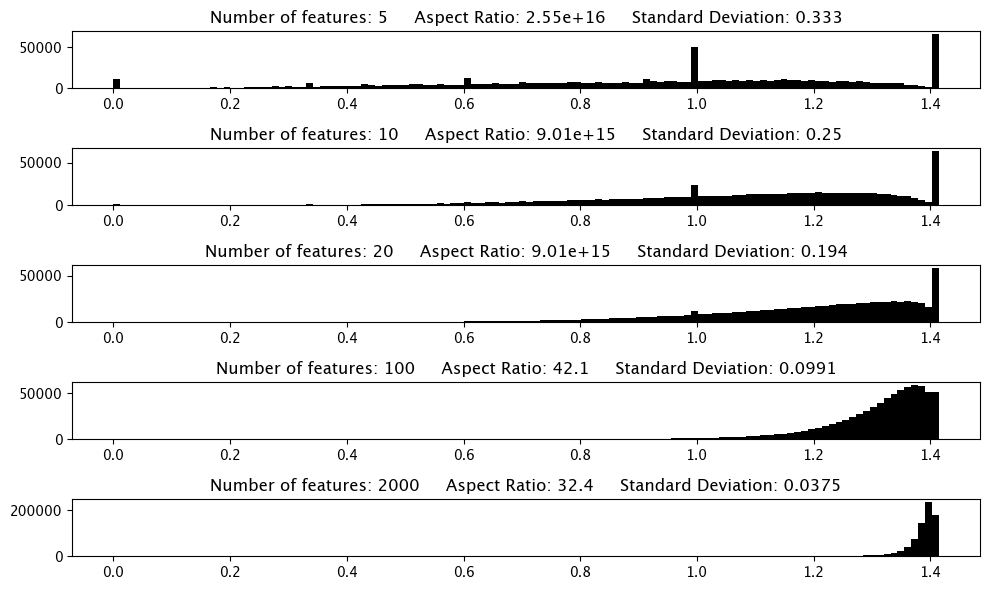
\includegraphics[width=\linewidth]{images/appendix_figs/dist_hist.png}
%    \caption{\small Higher dimensional data looks more like a regular simplex; an example in NLP. We plot the histogram of interpoint distances of a term frequency-inverse document frequency (tf-idf) vectorization of the BBC news dataset as we increase the number of features used. }\label{fig:NLP_simplex}
%\end{figure}

%\textcolor{red}{rework}
% It is also an intuitive property in practice: collecting more measurements and continually normalizing the resulting vector of measurements tends to push the minimum and maximum interpoint distances between data points closer together, see Figure \ref{fig:NLP_simplex} for a manifestation of this phenomenon in the NLP domain. 

\subsection{Empirical Comparison with UMAP}\label{app:umap1}
It is natural to ask whether related methods like UMAP suffer from the same failure modes that we point out for t-SNE in this work. 

In Figure \ref{fig:single_cell_umap}, we see how UMAP's output visualization is qualitatively unchanged between the given single cell dataset and its near-simplex impostor. However, unlike t-SNE, it does not display exact additive invariance, as the positioning of clusters changes. 
In Figure \ref{fig:amongus_umap}, we observe that UMAP, like t-SNE, displays extreme instability near the unit simplex.
In Figure \ref{fig:poison_umap}, we observe that UMAP's response to a single poison point is not as pronounced as that of t-SNE, but the injection of multiple poison points can still change the shape of the clusters significantly.

%Figure \ref{fig:single_cell_umap} demonstrates that UMAP has relatively similar behavior on

%see how other popular visualization methods such as UMAP fare with similar impostor inputs. This section shows that a similar issues persists.


\begin{figure}[h!]
    \centering
    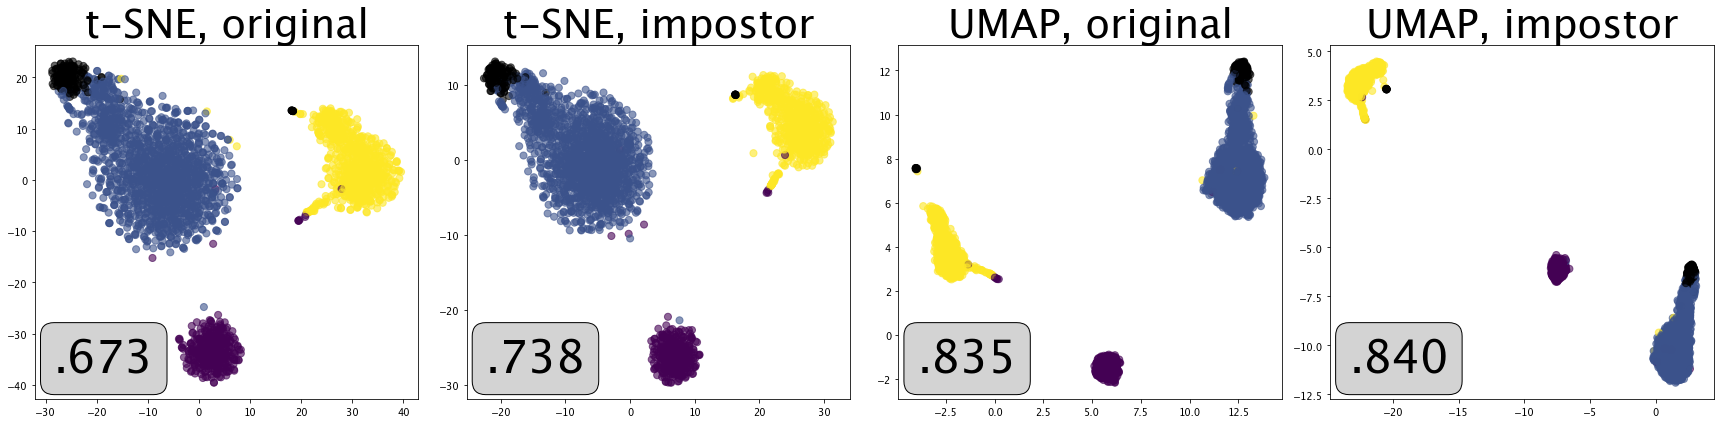
\includegraphics[width=\linewidth]{images/umap_figs/SINGLE_CELL.png}
    \vspace{-0.1in}
    \caption{UMAP on a real single-cell dataset versus (near simplex) impostor. The datasets and cluster partitions are those used in Figure \ref{fig:single_cell_false_pos}. Note that the bottom left number in each panel is the silhouette score of the embedding with respect to the clustering.}
    \label{fig:single_cell_umap}
\end{figure}

\begin{figure}[h!]
    \centering
    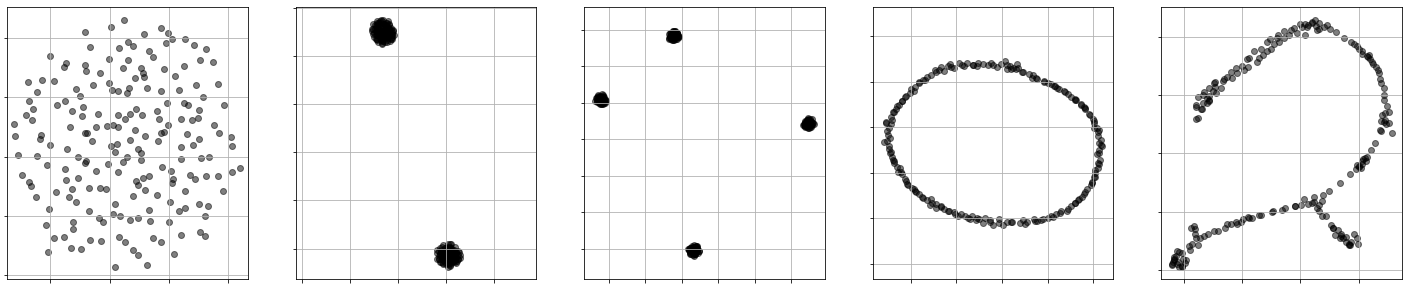
\includegraphics[width=\linewidth]{images/umap_figs/AMONGUS_.png}
        \vspace{-0.2in}
    \caption{\small Various different 2D UMAP visualizations produced by small adversarial perturbations of a 200-point unit regular simplex. These are the same datasets visualized in Figure \ref{fig:sameIn_diffOut}.}
    \label{fig:amongus_umap}
\end{figure}


\begin{figure}[h!]
    \centering
    %
\includegraphics[width=\linewidth]{images/umap_figs/poison_point_umap_.png}
    
\includegraphics[width=0.9\linewidth]{images/umap_figs/poison_point_umap_1000.png}
    \caption{{\small A comparison of t-SNE and UMAP's response to poison points, the original input being $1000$ points sampled from a mixture of two Gaussians in $2000$ dimensions. Notably, t-SNE, unlike UMAP, seems to have the property that even for very large datasets, a single poison point can destroy the cluster structure. UMAP generally has quite diverse responses to poison points. %For UMAP, the efficacy of a single poison point seems to have less impact % to have the behavior that, even for very large datasets, a single poison point can ruin the clustering, and large numbers of poison points can potentially create bridges between the clusters.   %The original dataset consists of 200 points from two slightly separated Gaussians. Each successive poison points is added by taking the mean of a random subset of \(15\) points.
    }}
    \label{fig:poison_umap}
\end{figure}




%INSERT FIGURE 1 AND 2 EQUIVALENT SHOWING T-SNE (REPRODUCED FROM FIG 1 and 2) AND UMAP PLOTS

\pagebreak
\subsection{Calinski-Harabasz Index}\label{sec:CHindex}
For an $n$-point dataset $X = \{x_1, \dots, x_n\} \subset \mathbb{R}^{n-1}$ and a partition of the dataset into non-empty clusters $C_1 \sqcup C_2 \sqcup \dots \sqcup C_k = [n]$ with $n > k > 1$, the Calinski-Harabasz Index is defined as the ratio of the distance between cluster centers to the  internal distance to a cluster's center. Let $E$ be the function from $S \subseteq [n]$ to $\mathbb{R}^{n-1}$ such that:
$$E(S) = \frac{1}{|S|}\sum_{i \in S} x_i.$$
Then the Calinski-Harabasz Index is\footnote{If the denominator and numerator are $0$, then $\text{CH}(X; C_{m \in [k]}) := 1$. If only the denominator is 0, then $\text{CH}(X; C_{m \in [k]}) := \infty$.}:
$$\text{CH}(X; C_{m \in [k]}) = \frac{\frac{1}{k-1}\sum_{m \in [k]} |C_m|\cdot \lVert E(C_m) - E([n])\rVert^2}{\frac{1}{n-k}\sum_{m \in [k]} \sum_{i \in C_m} \lVert x_i - E(C_m)\rVert^2}.$$

It ranges from $0$ to $\infty$ with a score of $\infty$ being assigned to perfectly clustered data, 1 to unclustered data and 0 to incorrectly clustered data. 

Now we provide an analogue to Theorem \ref{thm:unclustHammer} with respect to the Calinski-Harabasz Index:


\begin{theorem}
\label{thm:unclustHammerCH}
    Fix any $n > k > 1$, and $n$-point dataset ${X} \subset \mathbb{R}^{n-1}$ with partition $C_1 \sqcup \cdots \sqcup C_k = [n]$ such that $\textup{CH}({X}; C_{m\in[k]}) > 1$. For all $1 < \epsilon \leq \textup{CH}({X}; C_{m\in[k]})$, there exists $n$-point dataset ${X}_\epsilon \subset \mathbb{R}^{n-1}$ such that 
    $$\textup{CH}({X}_\epsilon; C_{m\in[k]}) = \epsilon, $$
    yet, for any $\rho \in [1, n-1]$:
    $${\TSNE}_\rho({X}) = {\TSNE}_\rho({X}_\epsilon).$$
\end{theorem}

\begin{corollary}
\label{cor:twoCluster_n_UnclusteredCH}
    For all $n \geq 4$ even, and partition $C_1 \sqcup C_2 = [n]$ such that $|C_1|=|C_2|=\frac{n}{2}$. There exist a sequence of $n$-point datasets in $\mathbb{R}^{n-1}$, $\{ {X}_\epsilon\}_{1 < \epsilon \leq \infty}$, with 
        $$\textup{CH}({X}_\epsilon; C_1, C_2) = \epsilon$$
    such that for any $\rho \in [1, n-1]$, $\bigcap_{1<\epsilon \leq \infty}\text{t-SNE}_\rho({X}_\epsilon)$ contains $n$-point dataset ${Y} \subseteq \mathbb{R}^2$ with
    $$\textup{CH}(Y; C_1,C_2) = \infty.$$ 
\end{corollary}

\begin{proof}[\textbf{Proof of Theorem \ref{thm:unclustHammerCH}}]
    First, let us assume that $\text{CH}(g(C); C_{m \in [k]}) < \infty$. Let $g$ be the function from Corollary \ref{cor:g_exists}, and $f(C) = \text{CH}(g(C); C_{m \in [k]})$. Note that $f$ is continuous whenever the denominator of $\text{CH}(\ \cdot\ ; C_{m \in [k]})$ is non-zero which is always the case for $C \in [0,1]$. Therefore, the image of $f$ on $[0,1)$ contains the interval $(f(1), f(0)] = (1, \text{CH}(X ; C_{m \in [k]})]$. Thus, for all $\epsilon \in (1, \text{CH}(X ; C_{m \in [k]})]$, there exists $C \in [0,1)$ such that $X_\epsilon = g(C)$ satisfies the hypothesis.

    If $\text{CH}(g(C); C_{m \in [k]}) = \infty,$ then $f$ is continuous on $(0,1)$ only. Thus for all ${\epsilon \in (1, \text{CH}(X ; C_{m \in [k]}))}$, there exists $C \in (0,1)$ such that $X_\epsilon = g(C)$ satisfies the hypothesis and for $\epsilon =\text{CH}(X ; C_{m \in [k]}))$, $X_\epsilon = X$ satisfies the hypothesis.
\end{proof}

For proof of Corollary \ref{cor:twoCluster_n_UnclusteredCH} see Appendix \ref{sec:proofs_clust}.

\subsection{Dunn Index}
\label{sec:Dunnindex}
For an $n$-point dataset $X = \{x_1, \dots, x_n\} \subset \mathbb{R}^{n-1}$ and a partition of the dataset into clusters $C_1 \sqcup C_2 \sqcup \dots \sqcup C_k = [n]$ with $|C_{m\in[k]}| > 1$, the Dunn index measures the ratio between the minimum inter-cluster distance and maximum intra-cluster distance. Specifically, the Dunn index is given by the expression\footnote{If the denominator and numerator are $0$, then $\text{DI}(X; C_{m \in [k]}) := 1$. If only the denominator is 0, then $\text{DI}(X; C_{m \in [k]}) := \infty$.}
$$\text{DI}(X; C_{m \in [k]}) = \frac{\min_{m,l \in [k], m\neq l, i \in C_m, j \in C_l} \lVert x_i - x_j \rVert}{\max_{m \in [k], i,j \in C_m} \lVert x_i - x_j \rVert}.$$


It ranges from $0$ to $\infty$ with a score of $0$ being assigned to incorrectly clustered data, $1$ to unclustered data, and $\infty$ to perfectly clustered data.

Now we restate Theorem \ref{thm:unclustHammer} with respect to the Dunn Index:

\begin{theorem}
\label{thm:unclustHammerDunn}
    Fix any $n > k > 1$, and $n$-point dataset ${X} \subset \mathbb{R}^{n-1}$ with partition $C_1 \sqcup \cdots \sqcup C_k = [n]$ such that $|C_{m\in[k]}| > 1$ and $\textup{DI}({X}; C_{m\in[k]}) > 1$. For all $1 < \epsilon \leq \textup{DI}({X}_\epsilon; C_{m\in[k]})$, there exists $n$-point dataset ${X}_\epsilon \subset \mathbb{R}^{n-1}$ such that 
    $$\textup{DI}({X}_\epsilon; C_{m\in[k]}) = \epsilon, $$
    yet, for any $\rho \in [1, n-1]$:
    $${\TSNE}_\rho({X}) = {\TSNE}_\rho({X}_\epsilon).$$
\end{theorem}

\begin{corollary}
\label{cor:twoCluster_n_UnclusteredDunn}
    For all $n \geq 4$ even, and partition $C_1 \sqcup C_2 = [n]$ such that $|C_1|=|C_2|=\frac{n}{2}$. There exist a sequence of $n$-point datasets in $\mathbb{R}^{n-1}$, $\{ {X}_\epsilon\}_{1 < \epsilon \leq \infty}$, with 
        $$\textup{DI}({X}_\epsilon; C_1, C_2) = \epsilon$$
    such that for any $\rho \in [1, n-1]$, $\bigcap_{1<\epsilon \leq \infty}\text{t-SNE}_\rho({X}_\epsilon)$ contains $n$-point dataset ${Y} \subseteq \mathbb{R}^2$ with
    $$\textup{DI}(Y; C_1,C_2) = \infty.$$ 
\end{corollary}

\begin{proof}[\textbf{Proof of Theorem \ref{thm:unclustHammerDunn}}]
    Let $g$ be the function from Corollary \ref{cor:g_exists}, and $f(C) = \text{DI}(g(C); C_{m \in [k]}).$ Fix $i,j \in [n]$ such that:
    $$\min_{m,l \in [k], m\neq l, i' \in C_m, j' \in C_l} \lVert x_{i'} - x_{j'} \rVert = \lVert x_i - x_j \rVert,$$
    and $t,r \in [n]$ such that:
    $$\max_{m \in [k], i',j' \in C_m} \lVert x_{i'} - x_{j'} \rVert = \lVert x_{r} - x_{t} \rVert,$$
    Then:
    $$f(C) = \frac{ \sqrt{(1-C)\cdot\lVert x_i - x_j \rVert+C}}{ \sqrt{(1-C)\cdot\lVert x_r - x_t \rVert+C}}.$$
    Thus the image of $f$ on $[0,1)$ is $(f(0), f(1)] = (1, \text{DI}(X; C_{m \in [k]})]$. Therefore, for all $\epsilon \in (1,\text{DI}(X; C_{m \in [k]})]$, there exists $C \in [0,1)$ such that $X_\epsilon = g(C)$ satisfies the hypothesis.
\end{proof}

For proof of Corollary \ref{cor:twoCluster_n_UnclusteredDunn} see Appendix \ref{sec:proofs_clust}.

\iffalse
\subsection{Davies–Bouldin index}
For an $n$-point dataset $X = \{x_1, \dots, x_n\} \subset \mathbb{R}^{n-1}$ and a partition of the dataset into clusters $C_1 \sqcup C_2 \sqcup \dots \sqcup C_k = [n]$ with $|C_{m\in[k]}| \geq 1$, the Davies–Bouldin index measures the average ratio of the distance between a cluster and a cluster centroid to the distance to the next closet cluster centroid. Let $E$ be as perviously defined in Appendix \ref{sec:CHindex} and fix $p,q \geq 1$. For $m,l \in [k]$ define:

$$S_m := \left( \frac{1}{|C_m|} \sum_{j \in C_m} \lVert x_j - E(C_m) \rVert_2^q\right)^{1/q}$$

and

$$M_{ml} = \lVert E(C_m) - E(C_l) \rVert_p.$$

Then the Davies–Bouldin index is:\footnote{If the denominator and numerator are 0, then $\frac{S_m+S_l}{M_{lm}} := ??$. If only the denominator is 0, then
$\frac{S_m+S_l}{M_{lm}} := \infty$.}

$$\bar{R}_{p,q}(X; C_{m\in[k]}) = \frac{1}{k} \sum_{m \in [k]} \max_{l \neq m} \frac{S_m +S_l}{M_{lm}}.$$

The index ranges from 0 to $\infty$ with a score of $0$ being assigned to perfectly clustered data, and $\infty$ to misclustered data. Let $\Dela \subset \mathbb{R}^{n-1}$ be a regular simplex of any side length. Then, the 

Now we restate Theorem \ref{thm:perturbhammer} with respect to the Davies-Bouldin index:

\fi








\subsection{Omitted Proofs}\label{sec:proofs_clust}

The main effort of this section will be to prove Lemma \ref{lem:image_of_tSNE}, which morally gives us Theorem \ref{thm:unclustHammer} and Theorem \ref{thm:perturbhammer}. In order to do this, we first introduce a number of technical lemmas which collectively show that t-SNE is invariant under additive and multiplicative scaling of the input.

\begin{lemma}\label{lem:unique_neighborhood} Let \(H(\cdot)\) denote the entropy function. For any $n>2$, \(X = \{x_1,\ldots,x_n\}\subset \mathbb{R}^{n-1}\) and \(\rho \in (1,n-1)\), there is a unique \(\sigma_i \geq 0\) that minimizes
\[\Big|  H(P_{\cdot |i}(X; \sigma_i) ) - \log_2 \rho \Big|.\]
\end{lemma}
\begin{proof}
   This follows easily from the fact that \(H(P_{\cdot |i}(X; \sigma))\) is a continuous, strictly increasing function of \(\sigma\) (see e.g.\ Lemma 4.2 of \citet{jeong2024convergence}), where \(\lim_{\sigma\to \infty}H(P_{\cdot |i}(X; \sigma)) = 
   \log_2(n-1)\) and \(H(P_{\cdot |i}(X; 0)) \in [0,\log_2(n-1)]\). %If \(\log_2 \rho \in (h, n-1)\), then there exists a unique \(\sigma_i\) achieving zero gap. Otherwise, the 
\end{proof}


\begin{definition}
   For any $n \geq 1$, dataset $X = \{x_1, \dots, x_n\} \subset \mathbb{R}^{n-1},$ and $C \geq 0$, define ${X_{+C} = \{x'_1, \dots, x'_n\} \subset \mathbb{R}^{n-1}}$ such that for all $i\neq j$ 
   $$\lVert x'_i-x_j' \rVert^2 = \lVert x_i-x_j \rVert^2 + C.$$
\end{definition}

\begin{lemma}\label{lem:X+C_exists}
    Fix any $n \geq 1$. For all $n$-point datasets $X = \{x_1, \dots, x_n\} \subset \mathbb{R}^{n-1}$ and $C \geq 0$, there exists $X_{+C} = \{x'_1, \dots, x'_n\} \subset \mathbb{R}^{n-1}$ such that for all $i\neq j$, $\lVert x'_i-x_j' \rVert^2 = \lVert x_i-x_j \rVert^2 + C$.
\end{lemma}
\begin{proof}
    Let $D$ be the inter-point squared distance matrix of $X$. Thus, the inter-point squared distance matrix of $X_{+C}$ is $D_{+C} = D + C\cdot (11^T-I_{n})$. By a famous theorem by \citet{schoenberg1938metric}, $X_{+C}$ is isometrically embeddable in $\mathbb{R}^{n-1}$ with respect to $\ell_2$ metric if and only if $\forall u \in \mathbb{R}^n$ with $u^T \vec{1} = 0$, $u^T D_{+C} u \leq 0$ holds. Indeed,
    $$u^T D_{+C} u = u^T D u + C\cdot(u^T\vec{1})(\vec{1}^T u) - C \cdot u^T u = u^T D u - C \cdot \lVert u \rVert^2 \leq 0,$$
    where the final inequality uses the fact that $D$ is embeddable.
\end{proof}

\begin{lemma}\label{lem:tSNE_additive_invariance}
    Fix any $n \geq 2$. For all $n$-point datasets $X \subset \mathbb{R}^{n-1}$, $\rho \in [1, n-1]$, and $C \geq 0$:
    $${\TSNE}_\rho(X) = {\TSNE}_\rho(X_{+C}).$$
\end{lemma}
\begin{proof}
    It is sufficient to show that the input affinity matrices for $X$ and $X_{+C}$ are identical. Indeed, for all $i,j \in [n], i\neq j$:
    \begin{align*}
        P_{i|j}(X) &= \frac{\exp\left(-\lVert x_i - x_j \rVert^2_2 / (2\sigma_i^2)\right)}{\sum_{k \neq i} \exp\left(-\lVert x_i - x_k \rVert^2_2 / (2\sigma_i^2)\right)} \\
        &= \frac{\exp\left(-(\lVert x_i - x_j \rVert^2_2+C) / (2\sigma_i^2)\right)}{\sum_{k \neq i} \exp\left(-(\lVert x_i - x_k \rVert^2_2+C) / (2\sigma_i^2)\right)} = P_{i|j}(X_{+C}).
    \end{align*}
\end{proof}



\begin{lemma}\label{lem:tSNE_multiplicative_invariance}
    Fix any $n \geq 2$. For all $n$-point datasets $X \subset \mathbb{R}^{n-1}$, $\rho \in (1, n-1)$, and $C > 0$:

    $${\TSNE}_\rho({X}) = {\TSNE}_\rho(C \cdot X).$$
\end{lemma}

\begin{proof}
 First note that for any dataset $X$ and its scaling $C\cdot X$, and all $\sigma_i\geq 0$, we have the following:
    \begin{align*}
        P_{j|i}(C\cdot X; C\cdot \sigma_i) = \frac{\exp(-C^2\cdot\lVert x_i-x_j\rVert^2/(2C^2\cdot\sigma_i^2))}{\sum_{k=1, k\neq j}^n \exp(-C^2\cdot\lVert x_i-x_k\rVert^2/(2C^2\cdot\sigma_i^2))} = P_{j|i}(X; \sigma_i).
    \end{align*}
Let \(H(\cdot)\) denote the entropy function. By the above, \({H(P_{\cdot | i}(X;\sigma_i)) = H(P_{\cdot | i}(C\cdot X;C\cdot \sigma_i))}\). Let $\sigma^*_i$ and correspondingly $\gamma^*_i$ be the (unique, per Lemma \ref{lem:unique_neighborhood}) neighborhood scalings that satisfy the perplexity condition for \(X\) and \(C\cdot X\) respectively (see Section \ref{sec:preliminaries}). Then \(\gamma_i^* = C\cdot \sigma_i^*\).

Therefore \(P_{\cdot |i}(C\cdot X; \gamma_i^*) = P_{\cdot |i}(C\cdot X; C\cdot \sigma_i^*) =P_{\cdot |i}(X; \sigma_i^*) \), yielding the result. 
\end{proof}

%Note that this additive invariance property of t-SNE was studied by \citet{lee2011, lee2014}.

The above lemmas give us the following useful corollary that will allow us to prove Lemma \ref{lem:image_of_tSNE}, Theorem \ref{thm:unclustHammer}, Theorem \ref{thm:unclustHammerCH}, and Theorem \ref{thm:unclustHammerDunn}.

\begin{corollary}\label{cor:g_exists}
    Fix any $n \geq 2$, and $X = \{x_1, \dots, x_n\} \subset \mathbb{R}^{n-1}.$ There exists a well-defined, continuous function $g: [0,1] \to \mathbb{R}^{n \times n-1}$ such that:
    $$C \mapsto ((1-C)\cdot X)_{+C},$$
    and for all $\rho \in [1, n-1]$ and $C \in [0,1):$
    $${\TSNE}_\rho(X) = {\TSNE}_\rho(g(C)).$$
    %Moreover, $g$ is such that for all $i \neq j, l \neq m \in [n]:$

    %$$\lVert x_i - x_j \rVert \leq \lVert x_l - x_k \rVert \implies \lVert g(C)_i - g(C)_j \rVert \leq \lVert g(C)_l - g(C)_k \rVert$$
\end{corollary}

\begin{proof}
    $g$ is well defined by Lemma \ref{lem:X+C_exists} and WLOG continuous since it continuously transforms the distances in $X$:
    $$\forall i,j \in [n], i\neq j, \hspace{1cm} \lVert g(C)_i - g(C)_j \rVert = \sqrt{(1-C)^2 \cdot \lVert x_i - x_j \rVert^2 + C}.$$
    Moreover, by Lemmas \ref{lem:tSNE_additive_invariance} and \ref{lem:tSNE_multiplicative_invariance}, for all $C \in [0,1):$
    $${\TSNE}_\rho(X) = {\TSNE}_\rho(g(C)).$$
\end{proof}

Using the additive and multiplicative invariance of t-SNE, we now prove Lemma \ref{lem:image_of_tSNE}:

%\todo[inline]{Redo labeling / maybe restatable?}
%
%\begin{lemma}
%    Fix any $n \geq 2$ and $\rho \in [1, n-1]$. For all $\epsilon > 0$, Let $S_\epsilon = \{ \mathcal{X}=\{x_1, \dots, x_n\} \subset \mathbb{R}^{n-1}: \forall i,j \in [n], \lVert x_i - x_j \rVert^2 \in [1-\epsilon, 1+\epsilon]\}$, then:
%    $${\TSNE}_\rho(n) = {\TSNE}_\rho(S_\epsilon).$$
%\end{lemma}

\begin{proof}[\textbf{Proof of Lemma \ref{lem:image_of_tSNE}}] 
    Fix any $\epsilon>0$. It suffices to show that ${\IMTSNE} \subseteq {\TSNE}_\rho(\Delta_\epsilon).$ Fix any $Y \in {\IMTSNE}$, there exists a $n$-point dataset $X = \{x_1,\ldots,x_n\} \subset \mathbb{R}^{n-1}$ such that:
    $$Y \in {\TSNE}_\rho(X).$$
    Using additive and multiplicative invariance, we will manipulate $X$ such that it is in $\Delta_\epsilon$ which by Lemma \ref{lem:tSNE_additive_invariance} and Lemma \ref{lem:tSNE_multiplicative_invariance} will not change the output. %Let $D_{\max} = \max_{i\neq j}\lVert x_i - x_ j \rVert$. WLOG, assume that $D_{\max} \neq 0$ otherwise $X_{+1} \in \Delta_\epsilon.$ 
    With respect to $X$, define $g:[0,1]\to\R^{n\times n-1}$ as in Corollary \ref{cor:g_exists}. Then for all $C \in [0,1):$
    $${\TSNE}_\rho(X) = {\TSNE}_\rho(g(C)).$$
    By the construction of $g,$ as $C$ approaches $1$, all inter-point distances in $g(C)$ approach $1$. Thus there must exist some $C \in [0,1)$ such that $g(C) \in \Delta_\epsilon$ which completes the proof.
\end{proof}

\iffalse
\begin{proof}[\textbf{Proof of Lemma \ref{lem:image_of_tSNE}}] 
    Fix any $\epsilon>0$. It suffices to show that ${\IMTSNE} \subseteq {\TSNE}_\rho(\Delta_\epsilon).$ Fix any $Y \in {\IMTSNE}$, there exists a $n$-point dataset $X = \{x_1,\ldots,x_n\} \subset \mathbb{R}^{n-1}$ such that:
    $$Y \in {\TSNE}_\rho(X).$$
    Using additive and multiplicative invariance, we will manipulate $X$ such that it is in $\Delta_\epsilon$ which by Lemma \ref{lem:tSNE_additive_invariance} and Lemma \ref{lem:tSNE_multiplicative_invariance} will not change the output. Let $D_{\max} = \max_{i\neq j}\lVert x_i - x_ j \rVert^2$ and $D_{\min} = \min_{i,j \in [n], i\neq j}\lVert x_i - x_ j \rVert^2$. WLOG, assume that $D_{\max} \neq 0$ otherwise $X_{+1} \in \Delta_\epsilon.$ Set $A = \frac{1}{2\epsilon}\big \lvert (1-\epsilon)D_{\max} - (1+\epsilon)D_{\min} \big \rvert$  and $B = \frac{1+\epsilon}{D_{\max} + A}.$ Note that since $A \geq 0$ and $D_{\max}>0$, $B$ is well defined and strictly greater than 0. Then the dataset $B \cdot (X_{+A}) = \{x'_1, \dots, x'_n\}$ exists by Lemma \ref{lem:X+C_exists} and is such that:
    $$\text{t-SNE}_\rho(X) = \text{t-SNE}_\rho(B \cdot (X_{+A}))$$
    by Lemma \ref{lem:tSNE_additive_invariance} and Lemma \ref{lem:tSNE_multiplicative_invariance}. Moreover, for all $i \neq j$:
    \begin{align*}
        \lVert x'_i - x'_j \rVert^2 &= \frac{1+\epsilon}{D_{\max}+A} \cdot (\lVert x_i - x_j \rVert^2+A) \leq  1+\epsilon,
    \end{align*}
    and
    \begin{align*}
        \lVert x'_i - x'_j \rVert^2 &\geq (1+\epsilon)\frac{D_{\min}+A}{D_{\max}+A}\\
        &\geq (1+\epsilon)\frac{D_{\min}+\frac{1}{2\epsilon}\big ( (1-\epsilon)D_{\max} - (1+\epsilon)D_{\min} \big )}{D_{\max}+\frac{1}{2\epsilon}\big ( (1-\epsilon)D_{\max} - (1+\epsilon)D_{\min} \big )}\\
        &\geq (1+\epsilon)\frac{(1-\epsilon)(D_{\max} - D_{\min})}{(1+\epsilon)(D_{\max} - D_{\min})} = 1-\epsilon,
    \end{align*}

    where the second inequality follows because $A \geq \frac{1}{2\epsilon}\big ( (1-\epsilon)D_{\max} - (1+\epsilon)D_{\min} \big ) > -D_{\max}.$
\end{proof}
\fi

Using the above lemmas, Theorem \ref{thm:unclustHammer}, Corollary \ref{cor:twoCluster_n_Unclustered}, and Theorem \ref{thm:perturbhammer} are proven.

\UnclustHammer*

\begin{proof}[\textbf{Proof of Theorem \ref{thm:unclustHammer}}]
    Let $g$ be the function from Corollary \ref{cor:g_exists}, and $f(C) = \bar{\mathcal{S}}(g(C); C_{m \in [k]}).$ Note that $f$ is continuous for $C \in [0,1]$ since $g$ is continuous, and $\bar{\mathcal{S}}(\ \cdot\ ; C_{m \in [k]})$ is continuous whenever for all $i\in[n]$, $a(i), b(i) \neq 0$ which follows from $\bar{\mathcal{S}}(X ; C_{m \in [k]})$ being well-defined and the definition of $g$. Therefore, the image of $f$ on $[0,1)$ contains the interval $(f(1), f(0)] = (0, \bar{\mathcal{S}}(X ; C_{m \in [k]})]$ (or if $\bar{\mathcal{S}}(X ; C_{m \in [k]}) \leq 0,$ $[\bar{\mathcal{S}}(X ; C_{m \in [k]}), 0)$). Thus, for all $\epsilon \in (0,1]$, there exists $C \in [0,1)$ such that $X_\epsilon = g(C)$ satisfies the hypothesis.
\end{proof}

Now we can prove Corollary \ref{cor:twoCluster_n_Unclustered}, Corollary \ref{cor:twoCluster_n_UnclusteredCH}, and Corollary \ref{cor:twoCluster_n_UnclusteredDunn} simultaneously: 

\iffalse
\todo[inline]{fix numbering of this corollary.}
\TwoClusterNUnclustered*
\fi

\begin{proof}[\textbf{Proof of Corollaries \ref{cor:twoCluster_n_Unclustered}, \ref{cor:twoCluster_n_UnclusteredCH}, and \ref{cor:twoCluster_n_UnclusteredDunn}}]
    The proof proceeds by showing a dataset and its output who have an average silhouette score of 1, Calinski-Harabasz index of $\infty$, and Dunn index of $\infty$, and then applies Theorem \ref{thm:unclustHammer}, Theorem \ref{thm:unclustHammerCH}, and Theorem \ref{thm:unclustHammerDunn} respectively. WLOG fix partition $C_1 \sqcup C_2 = [n]$ with $C_1=[1,n/2]$ and $C_2 = [n/2+1,n]$. Consider the $n$-point dataset, $X=\{x_1, \dots, x_n\} \subset \mathbb{R}^{n-1}$, such that for all $i \in C_1$, $x_i = \vec{0}$, and for all $i \in C_2$, $x_i = \vec{e_1}$.
    
    Routine calculations show that the conditional input affinities are:

    $$P_{i|j} = \begin{cases} 
          \frac{1}{\frac{n}{2}-1+\frac{n}{2}\exp\left(-\frac{1}{2\sigma^2_j} \right)} & i \in C(j), i \neq j \\
          \frac{\exp\left(-\frac{1}{2\sigma^2_j} \right)}{\frac{n}{2}-1+\frac{n}{2}\exp\left(-\frac{1}{2\sigma^2_j} \right)} & i \not\in C(j)\\
          0 & i = j.
       \end{cases}$$

    By symmetry, $\sigma_j = \sigma_i$ for all $i,j \in [n].$ Hence, let $\sigma$ be the neighborhood size for all $j \in [n]$ which is non-zero and well defined for $\rho \in [1, n-1].$ Thus the symmetrized input affinities are:

    $$P_{ij} = \begin{cases} 
          \frac{1}{\frac{n^2}{2}-n+\frac{n^2}{2}\exp\left(-\frac{1}{2\sigma^2} \right)} & i \in C(j), i\neq j \\
          \frac{\exp\left(-\frac{1}{2\sigma^2}\right)}{\frac{n^2}{2}-n+\frac{n^2}{2}\exp\left(-\frac{1}{2\sigma^2} \right)} & i \in C_1, j \in C_2 \\
          0 & i = j.
       \end{cases}$$

    Any set $Y = \{ y_1, \dots, y_n\} \subset \mathbb{R}$ is a global minimizer if $P_{ij} = Q_{ij}$ for all $i,j \in [n]$. In this case, this is achieved if $y_{i \in C_1} = 0$ and $y_{i \in C_2} = \sqrt{\exp\left( \frac{1}{2\sigma^2}\right) - 1}.$ Furthermore, since $Y$ can be isometrically embedded in $\mathbb{R}^d$ for all $d \geq 1$, this result holds for t-SNE embeddings of all dimensions. 

    To finish the proof note that for all $i \in [n]$ $a(i)=0$ when defined with respect to $Y$ and partition $C_1 \sqcup C_2.$
\end{proof}

\Perturbhammer*
\begin{proof}[\textbf{Proof of Theorem \ref{thm:perturbhammer}}]
    The proof is immediate by application of Lemma \ref{lem:image_of_tSNE}.
\end{proof}

\PoisonPoint*
\begin{proof}[\textbf{Proof of Theorem \ref{thm:poison_point}}]
Let \(J_n := \vec{1}_n \vec{1}_n^T\). To show the existence of \(X_0\) and \(X_1\), it suffices to write down their squared Euclidean interpoint distance matrices. Denote these \(D^2(X_0)\) and \(D^2(X_1)\) respectively. Define
   \[D^2(X_0) := J_n - I_n.\]
   This is a squared Euclidean distance matrix because it can be realized by a regular simplex (all points are equidistant). Now define
   \[D^2(X_1) := \begin{bmatrix}
       J_{n/2} - I_{n/2} & (1+r)  J_{n/2}   \\
       (1+r) J_{n/2}  &  J_{n/2} - I_{n/2}  
   \end{bmatrix}.\]
   This is also a squared Euclidean distance matrix because one can start with an embedding in \(\mathbb{R}\) where \(x_1 = \dots = x_{n/2} = 0\) and \(x_{n/2+1} = \dots = x_{n} = \sqrt{r}\), which has squared Euclidean distance matrix profile of
   \[\tilde D^2 = \begin{bmatrix}
       \vec{0}_{n/2}\vec{0}_{n/2}^T &  r  J_{n/2} \\
       r  J_{n/2}  &   \vec{0}_{n/2}\vec{0}_{n/2}^T 
   \end{bmatrix},\] 
   and then, recalling that the set of squared Euclidean distance matrices form a cone, one can argue that \(D^2(X_1) = \tilde D^2 + D^2(X_0)\) is also squared Euclidean.

   For any partition of \([n]\), it is clear that the silhouette score of \(X_0\) with respect to that partition is zero since all points are equidistant. As for \(X_1\), take \(r=2\) and observe that for \(C_1 = \{1,\dots, n/2\}\) and \(C_2 = \{n/2+1,\dots, n\}\), we have \(\bar{S}(X_1; C_1, C_2) = \frac{\sqrt{3} - 1}{\sqrt{3}} \approx 0.422.\)

Let \(X_0\) and \(X_1\) be Euclidean vector realizations of \(D^2(X_0)\) and \(D^2(X_1)\) each centered at the origin. Let \(x_0\) be the origin, and hence the mean of both datasets. Note that \(x_0\) will be equidistant to all the points in \(X_0\), and likewise with \(X_1\). 
\iffalse
To show this, it suffices to show that \(-\frac{1}{2}HD^2(X_0)H\) and \(-\frac{1}{2}HD^2(X_1)H\) are constant along the diagonal, where \(H = I_n - \frac{1}{n} J_n\). This is obvious for \(-\frac{1}{2}HD^2(X_0)H\). For \(-\frac{1}{2}HD^2(X_1)H\), observe:
\begin{align*}
    (HD^2(X_1)H)_{ii} &= \sum_{k=1}^n \sum_{j=1}^n H_{ik} H_{ji} D^2_{kj} \\
    &= D_{ii}^2(X_1) + \frac{1}{n^2}\sum_{k=1}^n \sum_{j=1}^n D_{kj}^2(X_1) - \frac{1}{n}\sum_{j=1}^n (D_{ij}^2(X_1) + D_{ji}^2(X_1)) 
\end{align*}
This quantity is constant for all \(i \in [n]\): the first term is always zero, the second term does not depend on \(i\), and the last term is constant because every row and column sums to \((n/2 - 1) + (1+r)(n/2)\).
\fi


To compute the distance of the mean \(x_0\) to other points, we make use of the fact that for all \(i\in [n]\)%\todo[inline]{I think that the normalization in the second equality should be something like $1/(n-1)^2$.}
\[\|x_0 - x_i\|^2 = \frac{1}{n} \sum_{j=1}^n \|x_0 - x_j\|^2 = \frac{1}{2}\cdot \frac{1}{n^2}\sum_{j=1}^n \sum_{k=1}^n \|x_k - x_j\|^2.\]
The resulting Euclidean distance matrices are as follows (where the distances corresponding to the appended point are written in the last row and column).%\todo[inline]{Why start using $J_n$ out of no where? Also note the red edits}
%\textcolor{red}{Is this obvious for \(X_1\cup x_0\)?}
 \[D^2(X_0\cup x_0) = \begin{bmatrix}
     J_{n} - I_n & (\frac{1}{2} - \frac{1}{2n})  \vec{1}_n \\
   (\frac{1}{2} - \frac{1}{2n})  \vec{1}_n^T  & 0
 \end{bmatrix},\]
 \[D^2(X_1\cup x_0) = \begin{bmatrix}
       J_{n/2} - I_{n/2 } & (1+r) J_{n/2}  & (\frac{1}{2} + \frac{r}{4 } - \frac{1}{2n}) \vec{1}_{n/2} \\
       (1+r) J_{n/2} &  J_{n/2} - I_{n/2}   & (\frac{1}{2} + \frac{r}{4 } - \frac{1}{2n}) \vec{1}_{n/2}  \\
       (\frac{1}{2} + \frac{r}{4 } - \frac{1}{2n}) \vec{1}_{n/2}^T & (\frac{1}{2} + \frac{r}{4 } - \frac{1}{2n}) \vec{1}_{n/2}^T & 0  
   \end{bmatrix}.\]
%\todo[inline]{Maybe move calculations of silhouette score to being before}
%\todo[inline]{Using square distances for silhouette which only uses non-squared distances. Should be (pls check for yourself) $\frac{\sqrt{3}-1}{\sqrt{3}} \approx 0.422$}
The key observation is that in both cases (recall the choice of \(r=2\)), for all \(i,j\in [n]\), \(\|x_i - x_0\|^2 < \|x_i-x_j\|^2\). %Thus, since we are in the \(\rho = 1\) regime, where \(P_{i|j} = \frac{1}{|N(j)|}\cdot \textbf{1}[i \in N(j)] \) where \(N(j) = \argmin_{l\in [n]\setminus\{j\}} \|x_j-x_l\|\), we have \(P_{ij} = 0\) for all \(i,j\in [n]\). 
By Lemma \ref{lem:rho_equal_one}, this implies that for \(\rho = 1\), \(P_{i|j}(X_0) = P_{i|j}(X_1) = 0\) for all \(i,j \in [n]\). In turn, \(P_{ij}(X_0) = P_{ij}(X_1) = 0\). Meanwhile \(P_{i|0}(X_0) = P_{i|0}(X_1) = 1/n\) (since \(x_0\) is equidistant from all other points) and \(P_{0|i}(X_0) = P_{0|i}(X_0) = 1\) for all \(i\in [n]\) (since \(x_0\) is every point's nearest neighbor). Thus both cases yield the same \(P\) matrix:
\[P(X_0\cup x_0) = P(X_1\cup x_0) =  \frac{1}{2(n+1)}\begin{bmatrix}
  \vec{0}_{n}\vec{0}_{n}^T & (1 + \frac{1}{n})\vec{1}_{n} \\
 (1 + \frac{1}{n})\vec{1}_{n}^T  & 0
\end{bmatrix}.\]
The equivalence of their loss landscapes follows immediately.
\end{proof}

\begin{lemma}\label{lem:rho_equal_one}  For \(\rho=1\) and any \(X = \{x_1,\dots, x_n\}\subset \mathbb{R}^D\),
\[P_{i|j}(X; \sigma^*_j) = \frac{1}{|N(j)|}\cdot \textbf{1}[i \in N(j)] \hspace{0.5cm}\text{where} \hspace{0.5cm} N(j) := \argmin_{k\in [n]\setminus\{j\}} \|x_k - x_j\|\]
\end{lemma}
\begin{proof}
    Note that \(\rho = 1\) corresponds to \(H(P_{\cdot|j}) = 0\), so we optimize the neighborhood size \(\sigma_j\) to minimize the entropy of the conditional affinities. This is done by taking \(\sigma_j = 0\). Recall
\[P_{i|j}(X; 0) = \lim_{\sigma_j \to 0} \frac{\exp(-\|x_i-x_j\|^2/2\sigma_j^2)}{\sum_{k=1, k\neq j}^n \exp(-\|x_k - x_j\|^2/2\sigma_j^2)} \]
    In the limit, only those \(x_k\) which are closest to \(x_j\) will dominate, i.e.\ \(x_k\) where \(k\in N(j)\). 
\end{proof}
%\begin{lemma} Let \(T \subset \mathbb{R}^d\).  \(\mathbb{E}_{(t,s)\sim T^2}[\|t - s\|^2] = 2\mathbb{E}_{t\sim T}[\|t - \mathbb{E}t\|^2] \).
%\end{lemma}




















\subsection{Impostor dataset construction}
\label{app:impostor_construction}

The construction of an impostor dataset based on an input dataset is done as follows.

\begin{algorithm}[H]
\caption{Impostor Dataset Creation}
\label{alg:impostor}
\begin{algorithmic}[1]
\Require Dataset $X = \{x_1, \ldots, x_n\}$ with at least two distinct points, and tolerance $\epsilon > 0$
%\Return Dataset $X_\epsilon = \{x_1', \ldots, x_n'\}$ such that $\mathrm{t\text{-}SNE}(X_\epsilon) = \mathrm{t\text{-}SNE}(X)$ and aspect ratio$(X_\epsilon) < 1+\epsilon$
\State Construct squared interpoint distance matrix of $X$, denote it by $D$
\State Form $D' \gets \frac{\epsilon}{\max_{i,j} D_{ij}} \cdot D + (11^\top - I_n)$
\State Run classical multidimensional scaling on $D'$ to obtain its Euclidean embedding $$X_\epsilon = \{x_1', \ldots, x_n'\} \subset \mathbb{R}^{n-1}.$$
\State \Return $X_\epsilon$
\end{algorithmic}
\end{algorithm}


%\newpage

\section{Appendix: Misrepresentation of Outliers}\label{sec:appendix_outliers}


\subsection{Additional Experiments}\label{sec:appendix_outliers_experiment}
We provide a comparison of t-SNE and PCA on the BBC news dataset. For ease of presentation, we take a three-cluster, \((n = 1204)\)-size subset (business, sports, tech) and we analyze what happens under injection of $120$ poison points versus $120$ far outliers. 

In both Figure \ref{fig:outliers_real_world} and Figure \ref{fig:bbc_appendix}, poison points are picked as follows: first we run a $k$-means algorithm on the original dataset; then, for each poison point, we pick one of the these means and $10$ random points of the dataset, and we average these two quantities (the idea is to connect the points in a way that contradicts the ground-truth three-clustering). We found \(k=2\) worked well. We pick outlier points as normal vectors centered at the mean of the dataset with variance \(32\) (the diameter of the original dataset is roughly \(1.5\)).
\begin{figure}[h!]
    \centering
    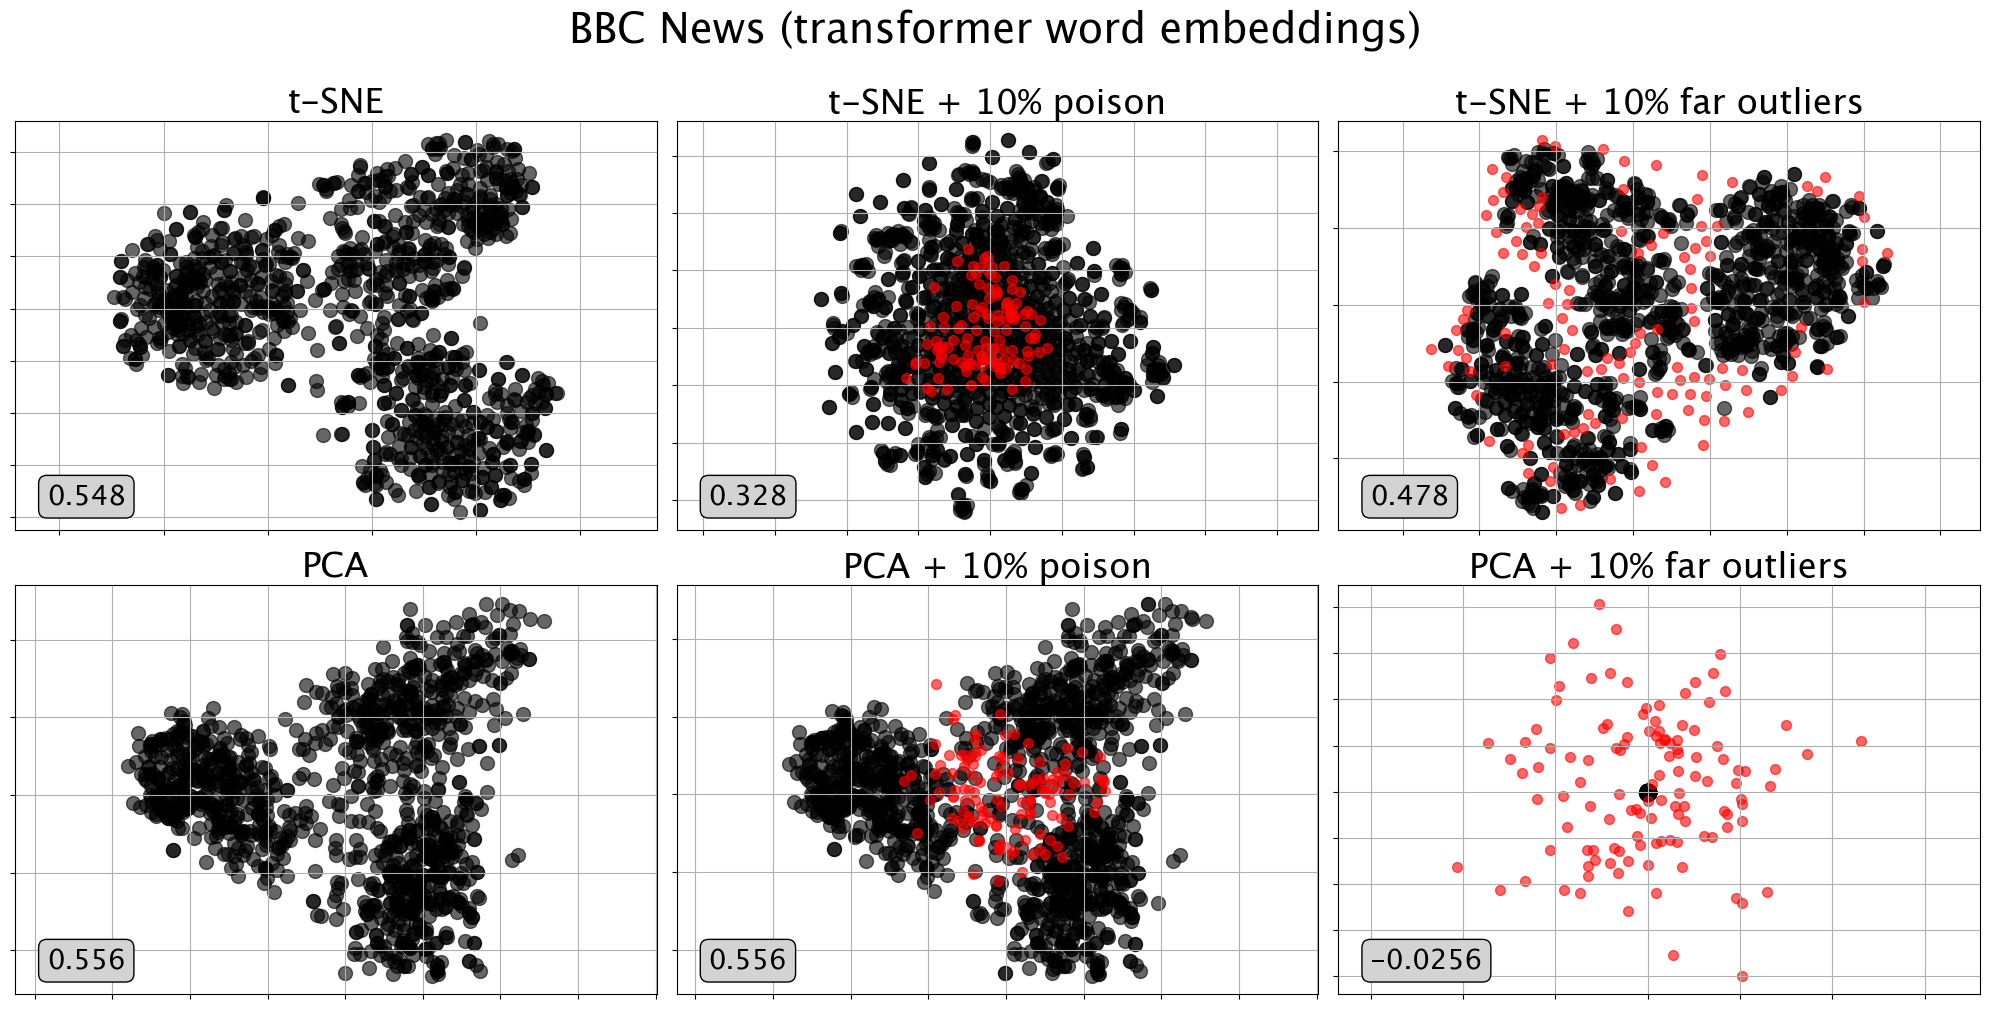
\includegraphics[width=\linewidth]{images/appendix_figs/bbc_appendix.png}
    \caption{\small t-SNE vs.\ PCA on poison points versus outlier points on a three-cluster subset of the BBC news dataset. The label on the bottom left is silhouette score of the plot (sans injected points) with respect to their ground-truth labels.}
    \label{fig:bbc_appendix}
\end{figure}


Below are additional experiments demonstrating t-SNE and PCA visualizations have divergent responses for single  poison point injection even as the size of the dataset increases.





\subsection{Empirical Comparison with UMAP}\label{app:umap2}

UMAP exhibits similar behavior to t-SNE when it comes to depicting far-away outliers. The main difference seems to be that UMAP tends to incorporate outliers deep into clusters, while t-SNE keeps them on the edge of clusters. As seen in Figure \ref{fig:outliers_real_world_UMAP} (right), this behavior can compromise the quality of clustering.

\begin{figure}[h!]
    \centering
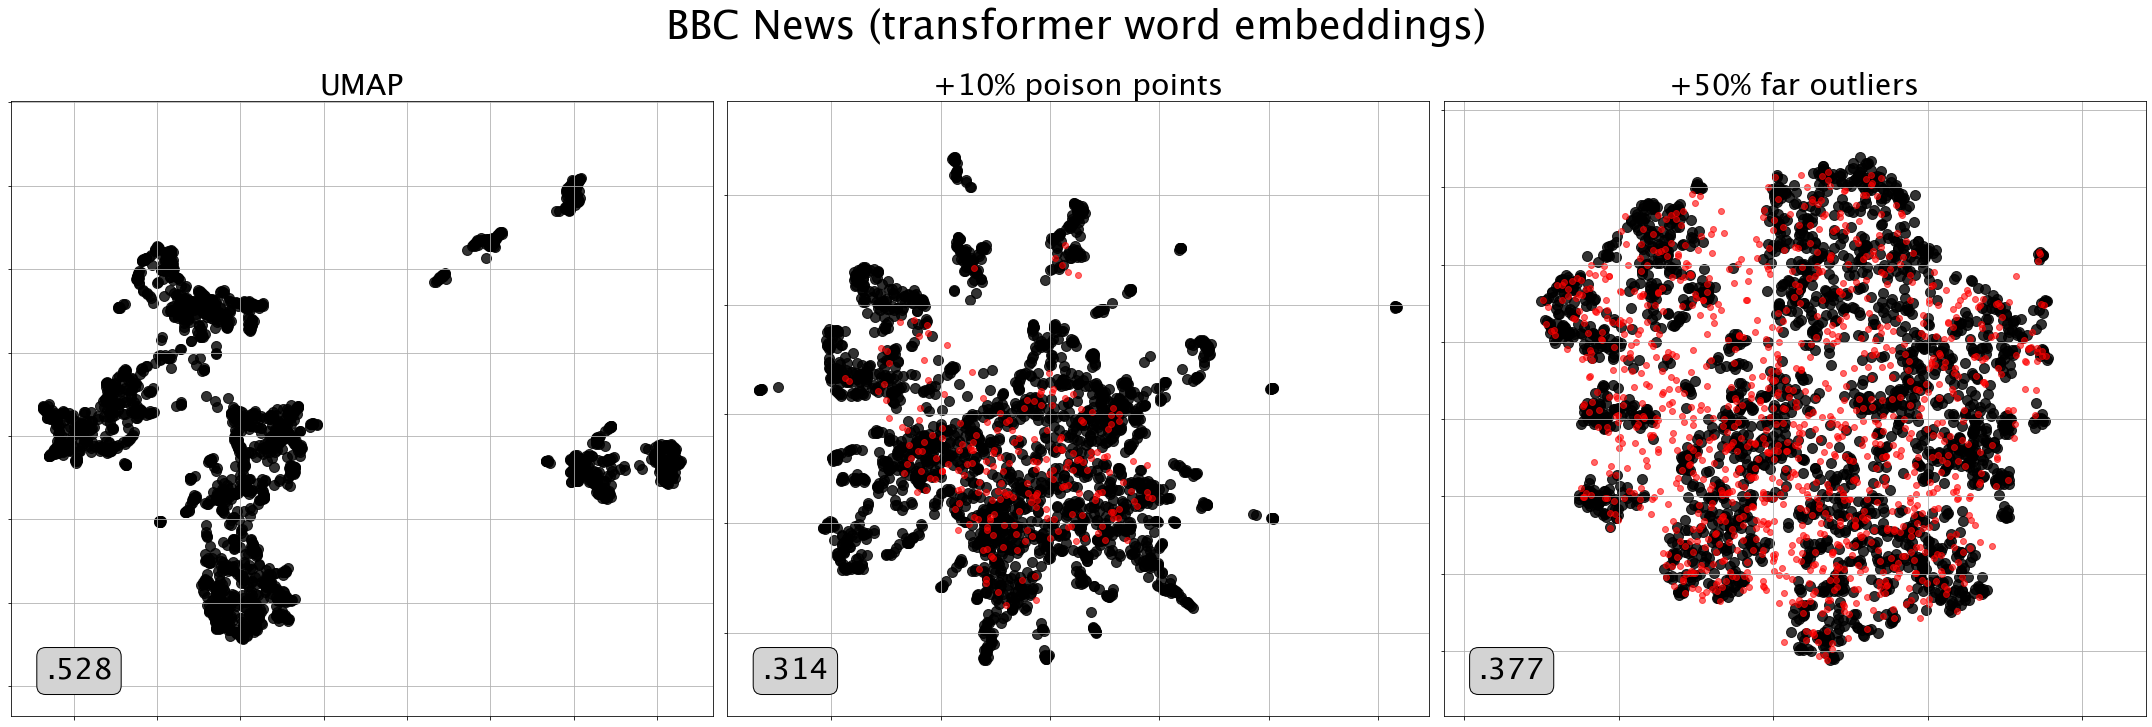
\includegraphics[width=\linewidth]{images/umap_figs/BBC_POISON_UMAP.png}
    \caption{\small UMAP in response to poison points versus \(\alpha\)-outliers on the BBC News dataset. The number in the bottom left of each panel is silhouette score with respect to the ground-truth. Compare with Figure \ref{fig:outliers_real_world}.}
\label{fig:outliers_real_world_UMAP}
\end{figure}


\begin{figure}[h!]
    \centering
    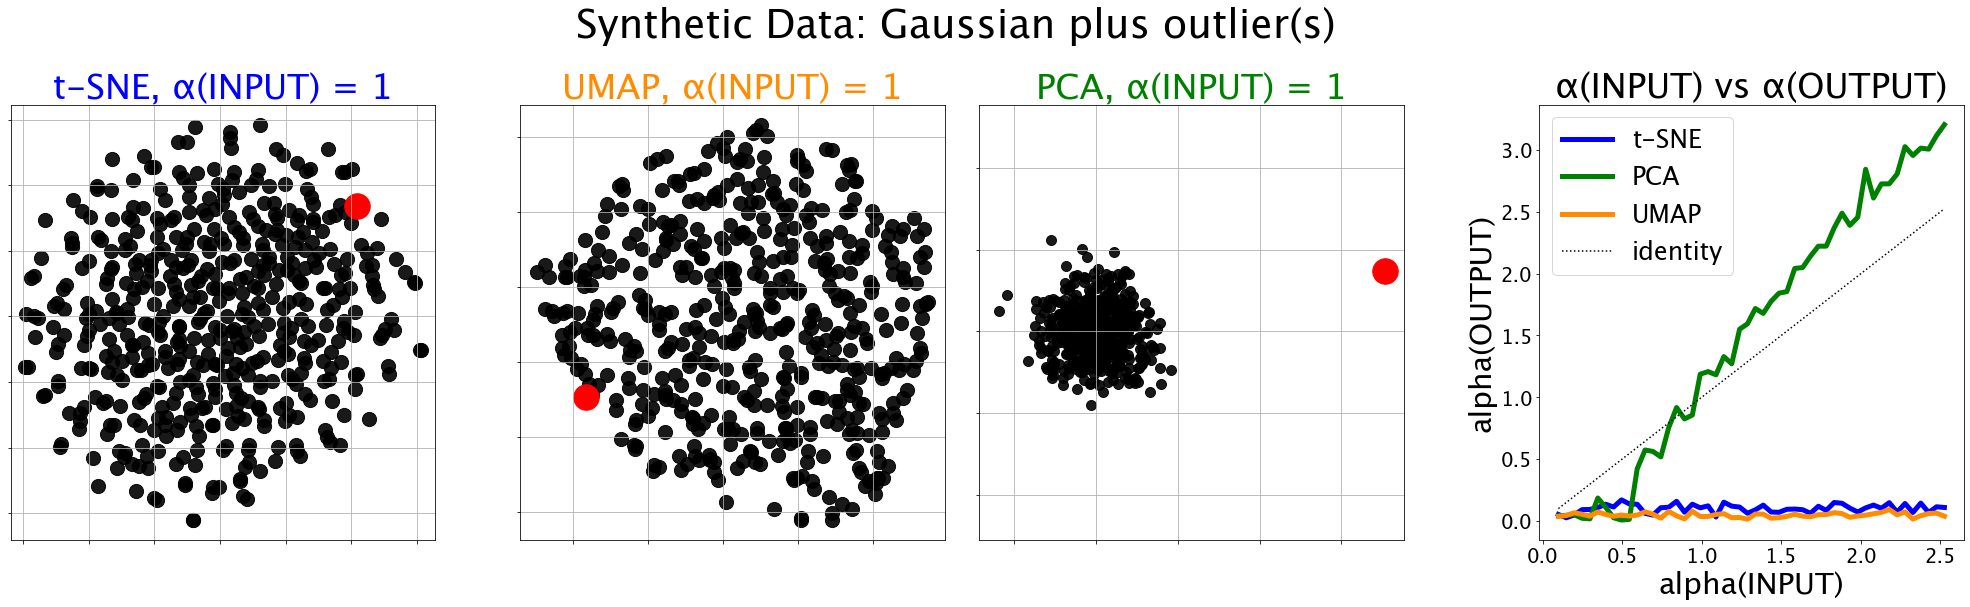
\includegraphics[width=\linewidth]{images/umap_figs/UMAP_outliers1.png}
    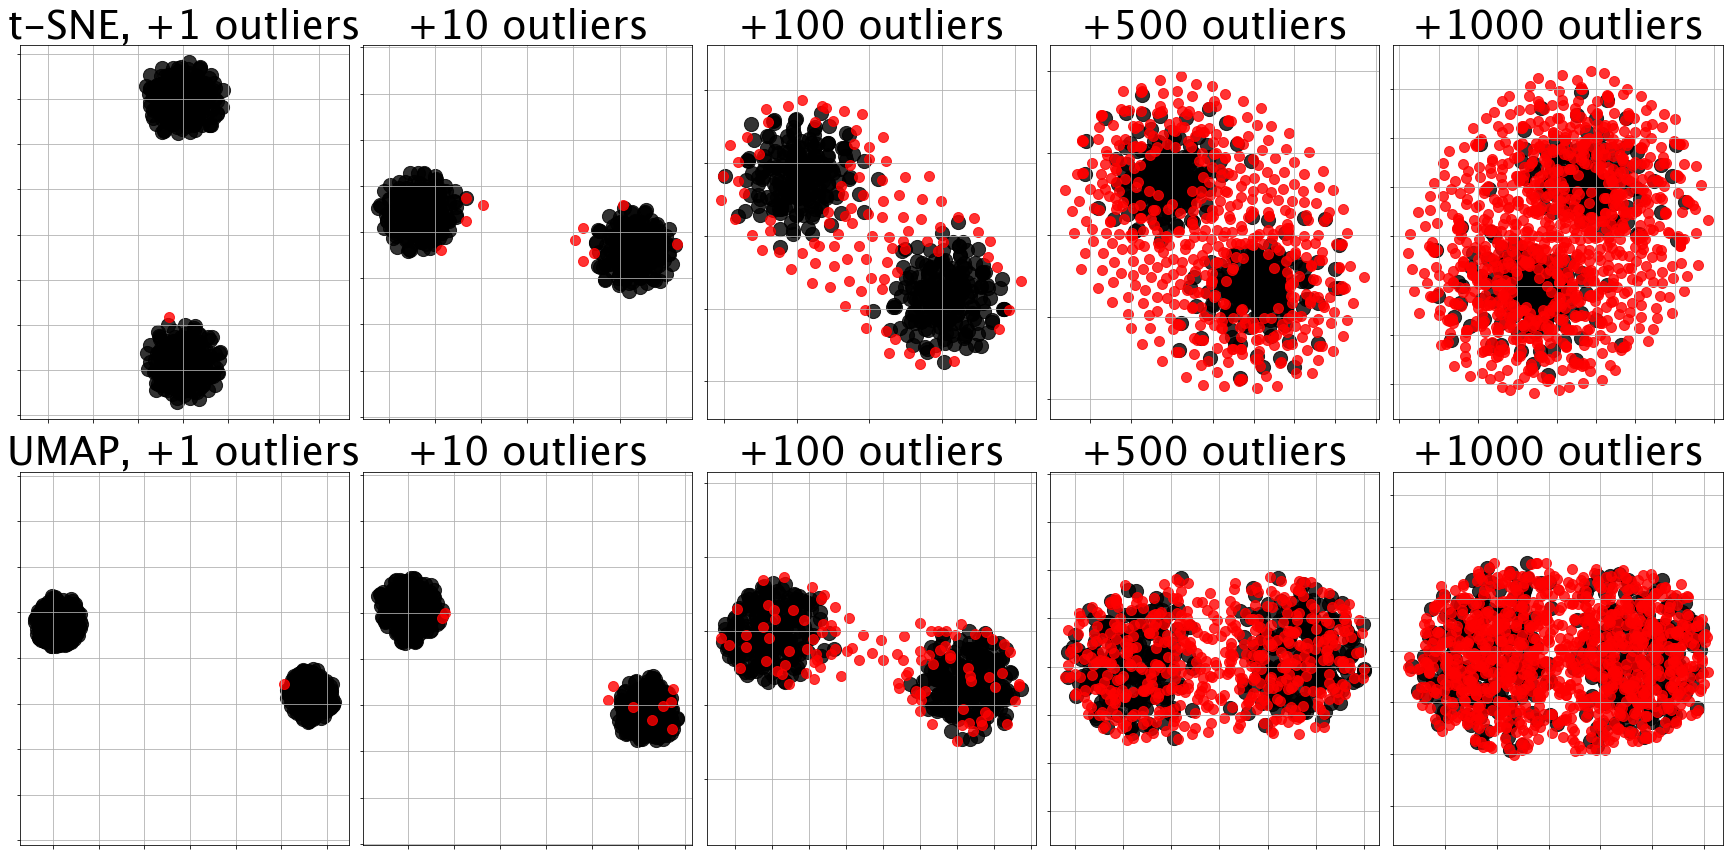
\includegraphics[width=\linewidth]{images/umap_figs/UMAP_outliers2.png}
    \caption{\small UMAP, like t-SNE, consistently suppresses faraway outliers. One salient difference between t-SNE and UMAP is that UMAP is more inclined to place outliers within clusters, whereas t-SNE often places them at the edge. Compare with Figure \ref{fig:outliers1}.}
    \label{fig:outliers_synthetic_UMAP}
\end{figure}




\newpage

\subsection{Omitted Proofs}

\begin{lemma}\label{lem:Qsum_bound} Fix $n\geq 2$ and \(Y = \{y_0,\ldots,y_{n-1}\} \subset \mathbb{R}^d\). Let ${\beta := \diam(Y\setminus \{y_0\})}$ and ${\gamma := \min_{j\in [n]} \|y_0-y_j\|}$. Then
\begin{align*}
    \sum_{i=1}^n Q_{0i} &\leq \frac{1}{2 + (n-2)\cdot \frac{1+\gamma^2}{1+\beta^2}} . %\\
   % &= \frac{1 +  D_Y^2}{2(1+D_Y^2 ) + (n-1)(1+\alpha^2 D_Y^2)} 
\end{align*}
\end{lemma}
\begin{proof}
    Let \(Z_0 = \sum_{i=1}^{n-1} \frac{1}{1+\|y_i-y_0\|^2}\) and \(Z_{1:n-1} = \sum_{i, j \in [n-1]: i\neq j}  \frac{1}{1+\|y_i-y_j\|^2}\). Then
    \[\sum_{i=1}^{n-1} Q_{0i} = \frac{Z_0}{2Z_0 + Z_{1:n-1}} = \frac{1}{2 + Z_{1:n-1}/Z_0}.\]
Now observe that
\begin{align*}
    \frac{Z_{1:n-1}}{Z_0} &= \frac{\sum_{i,j\in [n-1]:i\neq j} (1 + \|y_i-y_j\|^2)^{-1}}{\sum_{j=1}^{n-1} (1 + \|y_0 -y_j\|^2)^{-1}}  \\
 &\geq \frac{(n-1)(n-2)(1+\max_{i,j \in[n]} \|y_i-y_j\|^2)^{-1}}{(n-1)(1+\min_{j \in[n]} \|y_0-y_j\|^2)^{-1}}  \\
  &= \frac{(n-2)(1+\gamma^2)}{1+\beta^2}.  %\\
 % &= \frac{(n^2-n)(1+\beta^2)^{-1}}{n(1+\alpha^2)^{-1}}   \\
%  &= (n-1)\cdot \frac{1 + \alpha^2}{1 + \beta^2} .
    %&\geq \frac{(n^2-n)(1+ D_Y^2)}{n( 1 + \alpha^2 D_Y^2)}\geq (n-1)/\alpha^2 
\end{align*}
%Note that \(\min_{j\in [n]}\|y_0-y_j\|^2  \geq \alpha\max\{\beta,1\}\).
%{\color{red} Under new definition (margin-based) of $\alpha$-outlier, it is not obvious that $\alpha^2 = \min_{j \in [n]} \lVert y_0 - y_j \rVert^2$. Maybe do a case by case thing on whether $\diam > 1$. Also doesn't this margin definition add a factor $2$ somewhere to the inequality?}
Plugging this back into the previous equation gives the statement. 
\end{proof}

%\textcolor{red}{UNDER CONSTRUCTION}

\begin{lemma}\label{lem:r_split}
    Fix \(n\geq 2\) and \(Y = \{y_0,y_1,...,y_{n-1}\} \subset \mathbb{R}^d\). If \(Y\) is a \((\alpha, y_0)\)-outlier configuration such that $\alpha = \alpha(Y)$, then there exists $v \in \mathbb{R}^d$ such that for all $i \in [n]$:
    \[\|y_i-y_0\| \cdot \frac{ \alpha}{{1+\alpha}%\sqrt{1+\alpha^2}
    } \leq (y_i - y_0)\cdot v \leq \|y_i-y_0\|.\]
\end{lemma}

\begin{proof}
    Fix $i \in [n]$, let ${\beta := \diam(Y\setminus \{y_0\})}$, and WLOG let $y_0 = 0.$ Let $v$ be the unit vector defining the hyperplane as in Definition \ref{def:alpha_outlier}. Then by Cauchy-Schwarz, $(y_i-y_0) \cdot v \leq \| y_i-y_0 \|.$ To prove the other side of the inequality, we only need to lower bound the cosine of the angle between $y_i-y_0$ and $v$:
    $$(y_i - y_0)\cdot v = \| y_i - y_0 \| \cdot \cos(\angle({v, y_i})).$$
    Since $v$ is the maximum-margin hyperplane between $y_0=0$ and $Y\setminus \{y_0\}$, it holds that $u = v \cdot (\alpha \max\{1, \beta\})$ is in the convex hull of $Y\setminus \{y_0\}.$ Indeed, $\| u \| = \inf_{y \in \conv(Y\setminus \{y_0\})} \| y \|.$ Thus, we know that the closed ball $\overline{B_\beta (u)}$ contains $\conv(Y\setminus\{y_0\}).$ Therefore, there exists $t \in \mathbb{R}^d$ such that $\| t \| \leq \beta, u + t = y_i,$ and $u\cdot t \geq 0$. Hence
    $$\cos(\angle(v, y_i)) = \frac{v \cdot y_i}{\lVert y_i \rVert} = \frac{v\cdot(u+t)}{{\|u+t\|}} { \geq \frac{v\cdot u}{\|u\| + \|t\|}} \geq \frac{\alpha \max\{1,\beta\}}{{\alpha\max\{1,\beta\} + \max\{1, \beta\}}} \geq \frac{\alpha}{{1+\alpha}%\sqrt{1+\alpha^2}
    },$$
    %$$\cos(\angle(v, y_i)) = \frac{v \cdot y_i}{\lVert y_i \rVert} = \frac{v\cdot(u+t)}{\sqrt{\lVert u \rVert^2 + \lVert t\rVert^2 -2u \cdot t}} \geq \frac{\alpha \max(\beta, 1)}{\sqrt{\alpha^2 \max(\beta, 1)^2 + \beta^2}} \geq \frac{\alpha}{\sqrt{1+\alpha^2}},$$
    
   completing the proof.
\end{proof}


\OutlierAbs*
\begin{proof}
Fix $Y = \{y_0, y_1,\dots, y_{n-1}\} \in \IMTSNE$ and define \(\gamma = \min_i \|y_i-y_0\|\). WLOG, let \(y_0\) be the outlier point and assume $\gamma > 0$, otherwise the hypothesis goes through trivially.
    Since \(Y\) is stationary, \(\frac{\partial \mathcal{L}}{\partial y_0} = 0\). Pick \(v\) as in Lemma \ref{lem:r_split} and observe:
    \begin{align*}
        0 = \frac{\partial \mathcal{L}}{\partial y_0}\cdot v &= \sum_{i=1}^{n-1} \frac{(P_{i0} - Q_{i0})(y_0-y_i)\cdot v}{1 + \|y_0-y_i\|^2} \\
        &\leq -\frac{\alpha}{1+\alpha}\sum_{i=1}^{n-1}  P_{i0} \frac{\|y_0-y_i\|}{1 + \|y_0-y_i\|^2} + \sum_{i=1}^{n-1} Q_{i0} \frac{\|y_0-y_i\|}{1 + \|y_0-y_i\|^2}\\
     %   &\geq \frac{\alpha}{\textcolor{red}{1+\alpha}}\sum_{i=1}^{n-1}  P_{i0} \frac{\|y_0-y_i\|}{1 + \|y_0-y_i\|^2}- \sum_{i=1}^{n-1} Q_{i0} \frac{\|y_0-y_i\|}{1 + \|y_0-y_i\|^2}\\
        &\leq -\frac{\alpha}{1 + \alpha}  \frac{\gamma}{1+(\gamma+\beta)^2}\sum_{i=1}^{n-1} P_{i0}
        + \frac{\gamma + \beta}{1 + \gamma^2}\sum_{i=1}^{n-1} Q_{i0} \\
        &\leq  -\frac{\alpha}{1+\alpha}\frac{\gamma}{1+(\gamma+\beta)^2}\frac{1 + \sum_{i=1}^{n-1} P_{0|i}}{2n}
        + \frac{\gamma + \beta}{1 + \gamma^2}\frac{1}{2 + (n-2)\frac{1+\gamma^2}{1 + \beta^2}}
    \end{align*}
    \iffalse
    \begin{align*}
        0 = \frac{\partial \mathcal{L}}{\partial y_0}\cdot v &= \sum_{i=1}^{n-1} \frac{(P_{i0} - Q_{i0})(y_0-y_i)\cdot v}{1 + \|y_0-y_i\|^2} \\
        &\geq \frac{\alpha}{1+\alpha}\sum_{i=1}^{n-1}  P_{i0} \frac{\|y_0-y_i\|}{1 + \|y_0-y_i\|^2}- \sum_{i=1}^{n-1} Q_{i0} \frac{\|y_0-y_i\|}{1 + \|y_0-y_i\|^2}\\
     %   &\geq \frac{\alpha}{\textcolor{red}{1+\alpha}}\sum_{i=1}^{n-1}  P_{i0} \frac{\|y_0-y_i\|}{1 + \|y_0-y_i\|^2}- \sum_{i=1}^{n-1} Q_{i0} \frac{\|y_0-y_i\|}{1 + \|y_0-y_i\|^2}\\
        &\geq \frac{\alpha}{1 + \alpha}  \frac{\gamma}{1+(\gamma+\beta)^2}\sum_{i=1}^{n-1} P_{i0}
        - \frac{\gamma + \beta}{1 + \gamma^2}\sum_{i=1}^{n-1} Q_{i0} \\
  &\geq  \frac{\alpha}{1+\alpha}\frac{\gamma}{1+(\gamma+\beta)^2}\frac{1 + \sum_{i=1}^{n-1} P_{0|i}}{2n}
        - \frac{\gamma + \beta}{1 + \gamma^2}\frac{1}{2 + (n-2)\frac{1+\gamma^2}{1 + \beta^2}}
    \end{align*}
    \fi
where, in the fourth line, we use Lemma \ref{lem:Qsum_bound} and the fact that \(\sum_{i=1}^n P_{i|0} = 1\). Multiplying by $\frac{1+\gamma^2}{\gamma+\beta}\cdot \frac{2n}{1 + \sum_{i=1}^{n-1} P_{0|i}} > 0$ and rearranging, we get that:
    
%If the above expression is positive, this yields a contradiction with the stationary condition \(\partial \mathcal{L} / \partial y_0 = 0\). Therefore, the above expression must be non-positive. This implies %We can manipulate the expression as follows:


\begin{align*}
    \frac{\alpha}{{1+\alpha}} \cdot \frac{1+\gamma^2}{\gamma+\beta} \cdot \frac{\gamma}{1+(\gamma+\beta)^2} 
    &\leq \frac{1}{2 + (n-2)\cdot \frac{1+\gamma^2}{1+\beta^2}}\cdot \frac{2n}{1 + \sum_{i=1}^{n-1} P_{0|i}} \\
    &\leq \frac{1+\beta^2}{(n-2)(1+\gamma^2)}\cdot \frac{2n}{1 + \sum_{i=1}^{n-1} P_{0|i}} \\
    &= \frac{1+\beta^2}{1+\gamma^2}\cdot \Big(1 + \frac{2}{n-2}\Big)\cdot \frac{2}{1+\sum_{i=1}^{n-1} P_{0|i}}.
\end{align*}
Thus, by definition of \(\alpha\)-outlier configuration, $\gamma \geq \alpha \cdot \max\{\beta,1\}$:
\begin{align*}
    \Big(1 + \frac{2}{n-2}\Big)\cdot \frac{2}{1+\sum_{i=1}^{n-1} P_{0|i}} &\geq \frac{\alpha}{{1+\alpha}} \cdot \frac{\gamma}{\gamma+\beta} \cdot \frac{1+\gamma^2}{1+(\gamma+\beta)^2} \cdot \frac{1+\gamma^2}{1+\beta^2} \\ 
    &\geq \frac{\alpha}{{1+\alpha}}\frac{\gamma^3}{(\gamma+\beta)^3}\frac{1 + \gamma^2}{1+\beta^2} \\ 
    &\geq \frac{\alpha}{{1+\alpha}}\frac{\alpha^3\max\{\beta,1\}^3}{(\alpha\max\{\beta,1\}+\beta)^3}\frac{1 + \alpha^2\max\{\beta,1\}^2}{1+\beta^2} \\
    &\geq \frac{\alpha}{{1+\alpha}}\frac{\alpha^3}{(\alpha+\frac{\beta}{\max\{\beta,1\}})^3}\frac{1 + \alpha^2}{2} \\
    &\geq \frac{\alpha}{{1+\alpha}}\frac{\alpha^3}{(1+\alpha)^3}\frac{1 + \alpha^2}{2}\\
    &= {\frac{\alpha^4(1+\alpha^2)}{2(1+\alpha)^4}}. %\frac{\alpha^4\sqrt{1 + \alpha^2 }}{2(1+\alpha)^3}.
\end{align*}

Assume $\alpha \geq 3.26$ (or else the hypothesis holds trivially), then the above is lower-bounded by %${(\alpha^2 - 1)/{6}}$.
$0.1876 \alpha^2$.
Solving for $\alpha$ and observing that each $P_{0|i}$ is non-negative yields that:
\begin{align*}
    \alpha \leq \sqrt{\frac{1}{0.1876}\cdot\Big(1 + \frac{2}{n-2}\Big)\cdot \Big( \frac{{2}}{1+\sum_{i=1}^{n-1} P_{0|i}}\Big) } \leq \sqrt{\frac{2}{0.1876}\cdot\Big(1 + \frac{2}{n-2}\Big) } = 3.266 + o_n(1).
\end{align*}
\iffalse
\begin{align*}
    \alpha \leq \sqrt{1 + \Big(1 + \frac{2}{n-2}\Big)\cdot \Big( \frac{{12}}{1+\sum_{i=1}^{n-1} P_{0|i}}\Big) } \leq \sqrt{13 + \frac{24}{n-2} }.
\end{align*}
\fi
This concludes the proof.
\end{proof}